\documentclass[11pt]{article}
\usepackage[margin=0.86in]{geometry}
\usepackage[T1]{fontenc}
\usepackage{amsmath,amssymb,amsthm}
\usepackage{graphicx}
\usepackage[hidelinks]{hyperref}
\usepackage{microtype}

\newtheorem{theorem}{Theorem}
\newtheorem{lemma}[theorem]{Lemma}
\newtheorem{corollary}[theorem]{Corollary}
\newtheorem{remark}[theorem]{Remark}
\newcommand{\D}{\mathbb D}
\newcommand{\K}{\mathcal K}
\newcommand{\SA}{\mathcal{SA}}
\newcommand{\PsiH}{\widetilde\Psi_1^N}
\newcommand{\PsiA}{\widehat\Psi_{\mathbb A_q}^N}

\title{Unitary Conjugacy Destroys Minimality\\
of the Matrix Test-Function Families}
\author{fa\_banach\_001 / agent\_lane\_00}
\date{17 August 2026}

\begin{document}
\maketitle

\begin{center}
\fbox{\parbox{0.92\textwidth}{
\textbf{Claimed status: full negative resolution of both matrix-minimality
questions in arXiv:1109.3795, subject to human review.}
For every $N\ge2$, neither the normalized constrained-Hardy family
$\PsiH$ nor the normalized annulus family $\PsiA$ is minimal.  The scalar
case $N=1$ is known to be minimal, so both families are minimal exactly in
the scalar case.
}}
\end{center}

\section{The two source questions}

The paper asks whether the normalized matrix test family $\PsiH$ for
$\overline{\mathcal B}(H^\infty_1)^{N\times N}$ is minimal, and separately
conjectures minimality of its normalized matrix annulus Agler decomposition.
Here \emph{minimal} has the sense used in the cited scalar work: no proper
closed subfamily may be omitted while retaining the same class and
decompositions.

\begin{figure}[htbp]
\centering
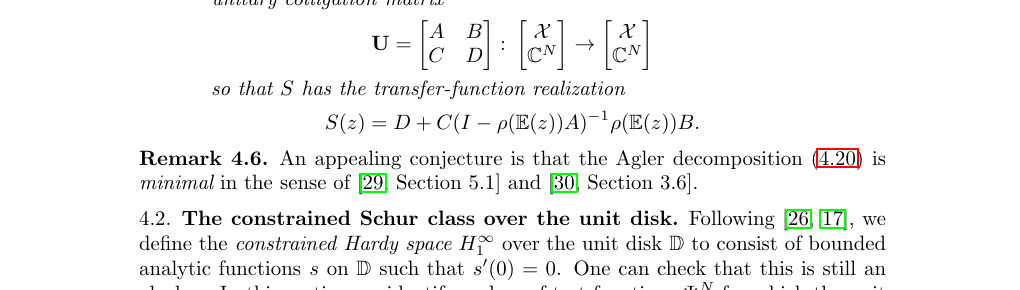
\includegraphics[width=0.90\textwidth]{figures/annulus_conjecture_crop.png}
\caption{The annulus minimality conjecture on PDF page 32.}
\end{figure}

\begin{figure}[htbp]
\centering
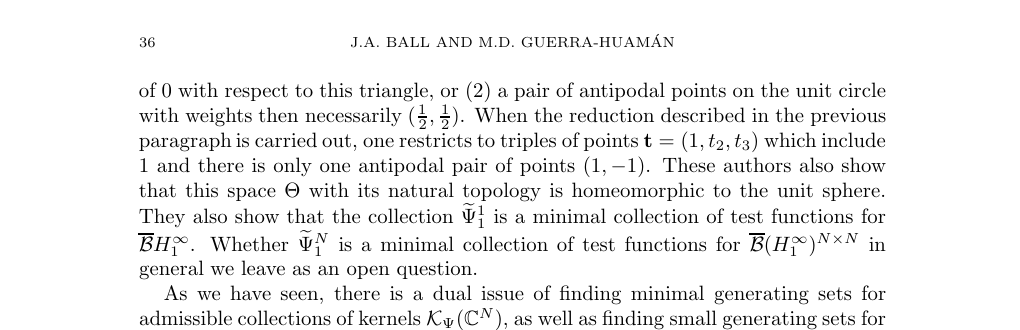
\includegraphics[width=0.90\textwidth]{figures/constrained_open_question_crop.png}
\caption{The constrained-Hardy open question on PDF page 36.}
\end{figure}

\section{A general symmetry obstruction}

For a matrix-valued test $\psi:\Omega\to M_N$ and a constant unitary
$U\in\mathcal U(N)$, write
\[
                       \psi^U(z)=U\psi(z)U^*.
\]

\begin{lemma}[Conjugate tests give the same constraint]\label{lem:constraint}
For every positive operator-valued kernel $K$, the test $\psi$ is a
contractive right multiplier on the source's Hilbert spaces if and only if
$\psi^U$ is.  Consequently, $\psi$ and $\psi^U$ impose identical
admissibility constraints.
\end{lemma}

\subsection*{Idea of the proof}

The paper tests contractivity against \emph{every} Hilbert--Schmidt-valued
function $X$.  Conjugating $\psi$ merely changes that dummy variable from
$X$ to $U^*X$.

\begin{proof}
Theorem 2.4 of the source says that admissibility is equivalent to positivity,
for every $X$, of
\begin{equation}\label{eq:testkernel}
 k_{X,\psi,K}(z,w)=\operatorname{tr}\!\left[
 X(w)^*\bigl(I-\psi(w)^*\psi(z)\bigr)X(z)K(z,w)\right].
\end{equation}
Since
\[
 I-\psi^U(w)^*\psi^U(z)
   =U\bigl(I-\psi(w)^*\psi(z)\bigr)U^*,
\]
we have
\[
                 k_{X,\psi^U,K}=k_{U^*X,\psi,K}.
\]
The substitution $X\leftrightarrow U^*X$ is a bijection on the class of all
test functions $X$, proving the equivalence.
\end{proof}

\begin{theorem}[Symmetry obstruction]\label{thm:symmetry}
Let $\Psi$ be a Hausdorff topological family of $M_N$-valued test functions.
Assume that $\psi\mapsto\psi^U$ is a homeomorphism of $\Psi$ and that
$\psi_0^U\ne\psi_0$ for some $\psi_0\in\Psi$.  Then $\Psi$ is not minimal:
there is a proper closed $C\subsetneq\Psi$ such that
\[
             \K_C(\mathcal E)=\K_\Psi(\mathcal E)
\]
for every auxiliary Hilbert space $\mathcal E$.  Hence
$\SA_C=\SA_\Psi$ and every general Agler-decomposition theorem valid for
$\Psi$ is valid with $C$.
\end{theorem}

\subsection*{Proof intuition}

Take a small open neighborhood of $\psi_0$ disjoint from its conjugate and
delete it.  Every deleted test still has a conjugate outside the deleted
set, and Lemma~\ref{lem:constraint} says that this retained conjugate imposes
the very same constraint.

\begin{proof}
Choose disjoint open neighborhoods $V$ of $\psi_0$ and $W$ of $\psi_0^U$,
and put
\[
 O=V\cap\{\psi:\psi^U\in W\},\qquad C=\Psi\setminus O.
\]
Then $O$ is nonempty and open, so $C$ is proper and closed.  Moreover
$\psi^U\in W\subset C$ for every $\psi\in O$.

Certainly $\K_\Psi(\mathcal E)\subseteq\K_C(\mathcal E)$.  Conversely, if
$K\in\K_C(\mathcal E)$ and $\psi\in\Psi$, either $\psi\in C$, or
$\psi\in O$ and the equivalent test $\psi^U$ lies in $C$.  In both cases
$K$ satisfies the $\psi$ constraint by Lemma~\ref{lem:constraint}.  Thus
$K\in\K_\Psi(\mathcal E)$, proving equality.  The Schur--Agler class is
defined solely through these admissible kernels, so it is unchanged.
\end{proof}

\section{The constrained-Hardy family}

\begin{lemma}\label{lem:noncentralH}
For every $N\ge2$, $\PsiH$ is invariant under constant unitary conjugation
and contains a noncentral test.
\end{lemma}

\begin{proof}
Unitary conjugation preserves the normalized constrained matrix Herglotz
class, its extreme points, the Cayley transform, and the normalization
$S(1)=I_N$.  Hence it acts homeomorphically on $\PsiH$.

We give an explicit noncentral member.  Let $P_j$ be the coordinate
rank-one projections.  For the first coordinate use the scalar measure
\[
 \mu_1=\tfrac12(\delta_1+\delta_{-1});
\]
for the second use
\[
 \mu_2=\tfrac13\bigl(\delta_{e^{i\pi/6}}+
 \delta_{e^{i5\pi/6}}+\delta_{e^{i3\pi/2}}\bigr).
\]
Both are probability measures with first moment zero, and both are extreme:
on their two or three support points, the mass and complex first-moment
equations uniquely determine the weights.  Their supports are disjoint.
Thus
\[
                         \mu=\mu_1P_1+\mu_2P_2
\]
is an extreme $2\times2$ constrained quantum probability measure.  Indeed,
in any positive convex decomposition of $\mu$, vanishing off its support
forces both summands onto that support; at each atom, rank-one support forces
the summand onto the same coordinate range; the two scalar extremality
statements then force equality.

The scalar Herglotz functions and Cayley transforms are
\[
 \frac{1+z^2}{1-z^2}\longleftrightarrow z^2,\qquad
 \frac{i+z^3}{i-z^3}\longleftrightarrow-i z^3.
\]
After the source's right-unitary normalization at $1$, the resulting member
of $\widetilde\Psi_1^2$ is
\[
                         \psi_0(z)=\operatorname{diag}(z^2,z^3).
\]
For $N>2$, append scalar extreme measures on pairwise-disjoint rotated
three-point supports.  This gives a normalized test whose first two entries
are still $z^2,z^3$.  Swapping the first two coordinates gives a distinct
unitary conjugate, so the test is noncentral.
\end{proof}

\begin{corollary}[Constrained-Hardy question]\label{cor:H}
For every $N\ge2$, $\PsiH$ is not a minimal collection of test functions
for $\overline{\mathcal B}(H^\infty_1)^{N\times N}$.
\end{corollary}

\begin{proof}
Apply Theorem~\ref{thm:symmetry} and Lemma~\ref{lem:noncentralH}.
\end{proof}

\section{The annulus family}

The reduced annulus tests in the source have the explicit form
\[
 \Phi_{[V],t}(z)=
 V\,\operatorname{diag}\bigl(\varphi_{t_1}(z),\ldots,
 \varphi_{t_N}(z)\bigr)V^*,
\]
and satisfy $\Phi_{[V],t}(1)=I_N$.  The family $\PsiA$ is therefore
invariant under conjugation: conjugation by $U$ replaces $V$ by $UV$.
For $N\ge2$, choose $t_1,t_2$ for which the scalar annulus tests are
distinct.  Taking $V=I$ produces a noncentral member.

\begin{corollary}[Annulus conjecture]\label{cor:A}
For every $N\ge2$, the matrix annulus family $\PsiA$ is not minimal.
In particular, the appealing conjecture in Remark 4.6 is false in every
genuinely matrix-valued size.
\end{corollary}

\begin{proof}
Apply Theorem~\ref{thm:symmetry}.  The resulting proper closed subfamily has
the same admissible kernels, hence the source's general theorem supplies
the same Agler decompositions using that subfamily.
\end{proof}

\section{Conclusion and scope}

The source cites scalar minimality for both examples.  Corollaries
\ref{cor:H} and \ref{cor:A} therefore give the exact classification:
\[
 \boxed{\text{each normalized family is minimal if and only if }N=1.}
\]
The obstruction concerns the source's families as stated.  It suggests the
natural repair: first quotient constant-unitary conjugacy, or choose a
topological slice for that action, before asking a refined minimality
question.

A bounded search of the run registry, exact question wording, title,
citations, and unitary-conjugacy terminology found no later explicit
resolution.  Novelty is provisional; the proof is self-contained.

\begin{thebibliography}{9}
\bibitem{BGH}
J. A. Ball and M. D. Guerra Huam\'an,
\emph{Test functions, Schur--Agler classes and transfer-function
realizations: the matrix-valued setting},
arXiv:1109.3795; Complex Analysis and Operator Theory \textbf{7}
(2013), 529--575,
\href{https://doi.org/10.1007/s11785-012-0218-x}
{doi:10.1007/s11785-012-0218-x}.

\bibitem{DP}
M. A. Dritschel and J. Pickering,
\emph{Test functions in constrained interpolation},
Transactions of the American Mathematical Society \textbf{364}
(2012), 5589--5604.
\end{thebibliography}

\end{document}
